%-------------------------------------------------------------------------------
\tikzset{fl/.style={ draw, fill = gray,rectangle,minimum size=3mm}}
\tikzset{sub/.style={ draw, shape border rotate=90, isosceles triangle,minimum size=8mm,yshift=-8mm}}
%-------------------------------------------------------------------------------
%-------------------------------------------------------------------------------
\chapter{Arbres AVL}
%-------------------------------------------------------------------------------
%-------------------------------------------------------------------------------
\thispagestyle{empty}
%-------------------------------------------------------------------------------
%-------------------------------------------------------------------------------
\begin{abstract}
On se propose ici d'implémenter la structure d'arbre binaire de recherche en assurant une hauteur logarithmique.
La structure choisie est celle définie par Georgy Adelson-Velsky and Evgenii Landis (d'où le nom AVL construit à partir des initiales) en 1962. On ajoute à un nœud l'indication de sa hauteur et on équilibre l'arbre à chaque opération.

On commencera par le dessin des arbres binaires afin de pouvoir visualiser les opérations.

La valeur des arbres sera réduite a la clé entière afin de simplifier l'étude mais la généralisation est immédiate.

On rappelle qu'un arbre est {\bf équilibré} si, pour tout nœud, la différence entre les hauteurs du fils droit et du fils gauche est au plus 1 en valeur absolue.

Le but de ce TP est de permettre d'obtenir des arbres équilibrés lors de des opérations sur les arbres binaires de recherche.
\end{abstract}
%-------------------------------------------------------------------------------
%-------------------------------------------------------------------------------
\begin{Exercise}[title = Préliminaire mathématiques]\it 

Montrer que si $a$ est un arbre équilibré de hauteur $h$ alors il contient au moins $F_{h+3}-1$ nœuds où $(F_n)$ est la suite de Fibonacci définie par $F_0=0$, $F_1=1$ et $F_{n+2} = F_{n+1}+F_n$.

En déduire que, pour un arbre équilibré de hauteur $h$ et de taille $n$, il existe un réel $A$ tel que 
$h \le A \log_2(n)$.
\end{Exercise}
%--------------------------------------------------------------------------
\begin{Answer}
On note ${\cal P}(h)$ la propriété :

 tout arbre équilibré de hauteur $h$ contient au moins $F_{h+2}-1$ nœuds.

Un arbre de hauteur 0 est un nœud de fils vides donc contient 1 nœud et $F_2-1=1$.

Un arbre de hauteur 1 est un nœud dont au moins un fils est non vide : il contient au moins 2 nœuds et $F_3-1=2$.
Ainsi ${\cal P}(0)$ et ${\cal P}(1)$ sont vraies.

On suppose que ${\cal P}(h-1)$ et ${\cal P}(h)$ sont vraies avec $h\ge 1$.

$a$ est un arbre équilibré de hauteur $h+1$.

Ses deux fils sont de hauteur $h$ au plus et au moins l'un des deux est de hauteur $h$.

Comme l'arbre est équilibré l'autre fils est de hauteur $h+\varepsilon$ avec $|\varepsilon| \le 1$ donc il est de hauteur $h-1$ au moins.

De plus les deux fils sont équilibrés donc l'un contient au moins $F_{h+2}-1$ nœuds et l'autre contient au moins $F_{h-1+2}-1$ nœuds. 

On en déduit que la taille de $a$ est minorée par $1+F_{h+2}-1+F_{h+1}-1=F_{h+3}-1$.

Ainsi ${\cal P}(h+1)$ est vrai donc la propriété est vraie pour tout arbre.

\medskip


Les racines de $X^2-X-1$ sont $\alpha=\frac{1+\sqrt 5}2$ et $\beta=\frac{1-\sqrt 5}2$ et $F_n=\frac 1{\sqrt 5}\bigl(\alpha^{n+1}-\beta^{n+1}\bigr)$ donc, pour un arbre équilibré on a $n \ge \frac 1{\sqrt 5}\bigl(\alpha^{h+3}-\beta^{h+3}\bigr)-1$. On en déduit

$\displaystyle \frac n{\alpha^h} \ge \frac {\alpha^3}{\sqrt 5}-\left(\frac \beta\alpha\right)^h\frac {\beta^3}{\sqrt 5}-\frac 1{\alpha^h}\ge  \frac {\alpha^3}{\sqrt 5}-\left(\frac \beta\alpha\right)^h\frac {\beta^3}{\sqrt 5}-1=F_2-1=1$

d'où $\alpha^h\le n$ puis $\displaystyle h \le \frac 1{\log_2(\alpha)}\log_2(n)$.
\end{Answer}
%--------------------------------------------------------------------------
%--------------------------------------------------------------------------
%--------------------------------------------------------------------------
\section{Dessin}
%--------------------------------------------------------------------------
%--------------------------------------------------------------------------
%-------------------------------------------------------------------------------
On souhaite  dessiner dessiner les arbres de telle manière que le parcours infixe consiste à lire les nœuds (et les feuilles)  de gauche à droite ; on impose aussi que les nœuds de même profondeur soient alignés horizontalement. On placera donc les nœuds sur une grille.

\medskip

Pour faire des représentations graphique on a besoin de la bibliothèque graphique.
%-------------------------------------------------------------------------------
\begin{lstlisting}
#load "graphics.cma";;
open Graphics;;
open_graph " 800x900";;
\end{lstlisting}
%-------------------------------------------------------------------------------
\begin{enumerate}
  \item La première ligne charge en mémoire le fichier de la bibliothèque.
  \item La deuxième ligne permet d'utiliser les fonctions de la bibliothèque directement : on écrit \type{set\_color} au lieu de \type{Graphics.set\_color}
  \item La troisième ligne ouvre une fenêtre graphique de 800 pixels de large et 900 pixels de haut. L'espace blanc avant le premier chiffre est obligatoire.
  
  L'origine est en bas à gauche.
\end{enumerate}
%-------------------------------------------------------------------------------
\begin{minipage}{0.5\textwidth}
\vspace{0pt}
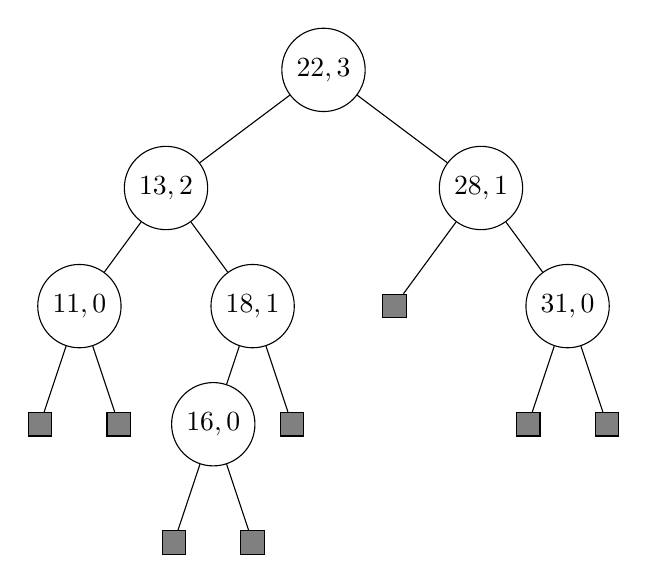
\begin{tikzpicture}[level distance =15mm]
\tikzstyle{level 1}=[sibling distance =4cm]
\tikzstyle{level 2}=[sibling distance =22mm]
\tikzstyle{level 3}=[sibling distance =10mm]
\tikzstyle{level 4}=[sibling distance =10mm]
\tikzstyle{every node}=[circle,draw]
\node {$22,3$}
 child {node{$13,2$}
        child {node{$11,0$}
               child {node[fl]{}}
               child {node[fl]{}}
              }
        child {node{$18,1$}
               child {node{$16,0$}
                      child {node[fl]{}}
                      child {node[fl]{}}
                     }
               child {node[fl]{}}
              }
       }
 child {node{$28,1$}
        child {node[fl]{}}
        child {node{$31,0$}
               child {node[fl]{}}
               child {node[fl]{}}
              }
       };
\end{tikzpicture} 
\end{minipage}
%-------------------------------------------------------------------------------
\begin{minipage}{0.50\textwidth}
\vspace{0pt}
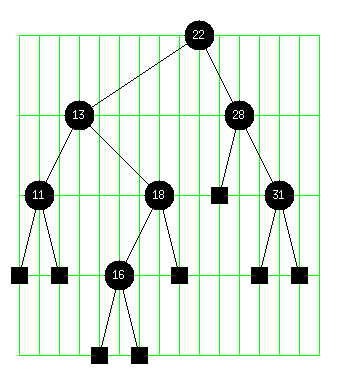
\includegraphics[scale=0.6]{arbre}
\end{minipage}
%-------------------------------------------------------------------------------
\medskip

La bibliothèque sait dessiner des segments de droites.

On a besoin des fonctions suivantes

\begin{itemize}
  \item \type{set\_color} sélectionne la couleur, les couleurs de base sont définies :
  
  \type{black, while, red, green, blue, yellow, cyan, magenta}.
  \item \type{set\_line\_width} sélectionne la largeur du trait.
  \item \type{moveto x y} déplace la position sans rien tracer vers $(x,y)$.
  \item \type{lineto x y} trace un trait depuis la position actuelle vers $(x,y)$ avec la couleur courante.
  \item \type{clear\_graph ()} efface le dessin courant.
  \item \type{close\_graph ()} ferme la fenêtre graphique.
\end{itemize}

\medskip

Pour voir ce que l'on dessine le programme ne doit pas clore tout de suite. On pourra employer une fonction qui attend un clic de la souris. Il est utile ensuite de fermer la fenêtre.
%--------------------------------------------------------------------------
\begin{lstlisting}
wait_next_event [Button_down];;
close_graph()
\end{lstlisting}
%--------------------------------------------------------------------------

Un exemple est donné dans le programme \type{dessin\_test.ml}.%--------------------------------------------------------------------------
%--------------------------------------------------------------------------
\begin{Exercise}\it Écrire une fonction qui permet la représentation du squelette d'un arbre.

On pourra donner comme paramètre les coordonnées du point supérieur gauche et considérer que les pas de la grille  horizontaux (\type{dX}) et verticaux (\type{dY}) sont des variables globales (de valeurs 20 et -80, par exemple car on veut aller vers le bas).
\end{Exercise}
%--------------------------------------------------------------------------
\begin{Answer}
On écrit une fonction auxiliaire qui reçoit les coordonnées du points supérieur gauche du rectangle contenant l'arbre et qui renvoie la nouvelle abscisse pour la suite ainsi que l'abscisse de la racine.
\begin{lstlisting}
let rec squelette arbre x0 y0 =
  set_color black;
  match arbre with
  |Vide -> x0, x0
  |Noeud(k, g, r, d) -> let xrg, xbg = squelette g x0 (y0 - dY) in
                        let xr = xbg + dX in
                        let xrd, xbd = squelette d (xr + dX) (y0 - dY) in
                        moveto xrg (y0 - dY);
                        lineto xr y0;
                        lineto xrd (y0 - dY);
                        xr, xbd;;
\end{lstlisting}
\newpage
\end{Answer}
%--------------------------------------------------------------------------%--------------------------------------------------------------------------
Une idée possible est de dessiner l'arbre gauche en décalant l'ordonnée d'origine d'un pas vers le bas.
Pour savoir où placer la racine, la fonction doit renvoyer le bord droit du dessin du fils. 

On trace alors le fils droit en décalant encore vers la droite.

Pour tracer les segments depuis la racine, il faut aussi recevoir l'abscisse des racines des fils : la fonction de dessin, en plus de dessiner l'arbre devra renvoyer l'abscisse de la racine et l'abscisse du bord droit

\medskip

Des fonctions supplémentaires possibles sont
%--------------------------------------------------------------------------
\begin{itemize}
  \item \type{fill\_rect x0 y0 larg haut} qui dessine un rectangle dont le point en bas à gauche est aux coordonnées $(x_0,y_0)$, de largeur \type{larg} et de hauteur \type{haut}. Le rectangle est rempli par la couleur courante.
%--------------------------------------------------------------------------
  \item \type{fill\_circle x0 y0 r} qui dessine un cercle rempli par la couleur courante, de centre $(x_0,y_0)$ et de rayon \type{r}.
%--------------------------------------------------------------------------
  \item \type{draw\_string texte} qui écrit un texte avec la couleur courante depuis la position actuelle (elle correspond au point en bas à gauche).
\end{itemize}
%--------------------------------------------------------------------------
Par exemple pour dessiner un disque rouge, centré en $(x,y)$, de rayon $r$ et marqué d'un chiffre $n<100$, on peut écrire
%--------------------------------------------------------------------------
\begin{lstlisting}
let disqueRouge x y r n =
  set_color red; 
  fill_circle x y r;
  set_color white;
  if n < 10 
  then moveto (x - 2) (y - 5)
  else moveto (x - 6) (y - 5);
  draw_string (string_of_int n);;
\end{lstlisting}
%--------------------------------------------------------------------------
%--------------------------------------------------------------------------
\begin{Exercise}\it Écrire une fonction qui permet la représentation des nœuds d'un arbre.

On représentera les feuilles par des carrés de côté 16 et les nœuds internes par des disques de rayon 15.
\end{Exercise}
%--------------------------------------------------------------------------
\begin{Answer}
On s'inspire du squelette.
\begin{lstlisting}
let cote = 16
let rayon = 15;;

let dessinNoeud arbre x y =
(* Dessin de la racine d'un arbre à la position (x,y)*)
match arbre with
|Vide -> set_color black;
fill_rect (x-cote/2) (y-cote/2) cote cote
|Noeud(_, n, _ , _) -> 
set_color black;
fill_circle x y rayon;
set_color white;
if n < 10 then moveto (x - 2) (y - 5)
else moveto (x - 6) (y - 5);
draw_string (string_of_int n);;


let rec noeuds arbre x0 y0 =
match arbre with
|Vide -> dessinNoeud Vide x0 y0; x0
|Noeud(g, n, d, h) -> 
(let xg = noeuds g x0 (y0 + dY) in
let xr = xg + dX in
let xd = noeuds d (xr + dX) (y0 + dY) in
dessinNoeud arbre xr y0 ;
\end{lstlisting}
\end{Answer}
%--------------------------------------------------------------------------
%--------------------------------------------------------------------------
\begin{Exercise}\it En déduire un tracé de l'arbre : les segments ne doivent pas passer par dessus les nœuds.

Peut-on faire la même chose en un seul passage ?
\end{Exercise}
%--------------------------------------------------------------------------
\begin{Answer}
On dessine le squelette avant les nœuds.
\begin{lstlisting}
open_graph " 800x900";;
squelette a0 x0 y0;;
noeuds a0 x0 y0;;
wait_next_event [Button_down];;
close_graph ();;
\end{lstlisting}
%--------------------------------------------------------------------------
\begin{lstlisting}
let dessin arbre x0 y0 = 
  let rec auxDessin arbre x y = 
  match arbre with
  |Vide -> (x + dX, x)
  |Noeud(g, n, d, h) -> 
    let (xg, xrg) = auxDessin g x (y + dY) in                     
    let (xd, xrd) = auxDessin d (xg+dX) (y + dY) in
    set_color black;
    moveto xrg (y + dY);
    lineto xg y;
    lineto xrd (y + dY);
    dessinNoeud g xrg (y + dY);
    dessinNoeud d xrd (y + dY);
    (xd, xg) in
    let max, xr = auxDessin arbre x0 y0 in 
  dessinNoeud arbre xr y0;
  wait_next_event [Button_down];;
\end{lstlisting}
\newpage
\end{Answer}
%-------------------------------------------------------------------------------
%-------------------------------------------------------------------------------
\section{Équilibrage}
%--------------------------------------------------------------------------
%-------------------------------------------------------------------------------
On considère un type d'arbre binaires de recherche que l'on a augmenté de l'indication de la hauteur (en quatrième argument de la hauteur).

Le type utilisé sera 
\begin{lstlisting}
type arbreAVL = Vide|Noeud of  arbreAVL * int * arbreAVL * int;;
\end{lstlisting}

Les constructions devront s'assurer que la hauteur est bien la valeur indiquée.
%-------------------------------------------------------------------------------
%-------------------------------------------------------------------------------
\subsection{Premières fonctions}
%--------------------------------------------------------------------------
\begin{Exercise}\it 
Écrire une fonction qui teste l'appartenance d'une valeur à un arbre.

Il s'agit de transcrire simplement la fonction du cours.
\end{Exercise}
%--------------------------------------------------------------------------
\begin{Answer} 
\begin{lstlisting}
let rec chercher n arbre = 
  match arbre with
  |Vide -> false
  |Noeud(g, r, d, h) when (n = rx) -> true
  |Noeud(g, r, d, h) when (n < r) -> chercher n g
  |Noeud(g, r, d, h) -> chercher n d;;
\end{lstlisting}
\end{Answer}
%--------------------------------------------------------------------------
%--------------------------------------------------------------------------
\begin{Exercise}\it 
Écrire une fonction qui crée une feuille à partir d'une valeur du nœud.
\end{Exercise}
%--------------------------------------------------------------------------
\begin{Answer} 
\begin{lstlisting}
let feuille r =  Noeud(Vide, r, Vide, 0);;
\end{lstlisting}
\end{Answer}
%--------------------------------------------------------------------------
%--------------------------------------------------------------------------
\begin{Exercise}\it 
Écrire une fonction \type{ht} qui renvoie la hauteur d'un arbre.

La fonction doit renvoyer $-1$ dans le cas d'un arbre vide.
\end{Exercise}
%--------------------------------------------------------------------------
\begin{Answer} 
\begin{lstlisting}
let ht arbre = 
  match arbre with
  |Vide -> -1
  |Noeud(g, r, d, h) -> h;;
\end{lstlisting}
\end{Answer}
%--------------------------------------------------------------------------
%--------------------------------------------------------------------------
\begin{Exercise}\it 
Écrire une fonction \type{cons g n0 d} avec $n_0$ valeur et $g$ et $d$ deux arbres AVL (non nécessairement équilibrés) qui renvoie un arbre AVL construit avec les paramètres (fils gauche, racine et fils droit respectivement).
\end{Exercise}
%--------------------------------------------------------------------------
\begin{Answer} 
\begin{lstlisting}
let cons g n0 d = 
  let hg = ht g in
  let hd = ht d in
  let h = (max hg hd) + 1 in 
  Noeud(g, n0, d, h);;
\end{lstlisting}
\end{Answer}
%--------------------------------------------------------------------------
\newpage
%-------------------------------------------------------------------------------
\subsection{Rotations}
%--------------------------------------------------------------------------
Lors de l'ajout ou le retrait d'un élément peut perturber l'équilibre.

Dans l'exemple ci-dessous, ou ajoute la valeur 5.
%-------------------------------------------------------------------------------
\[
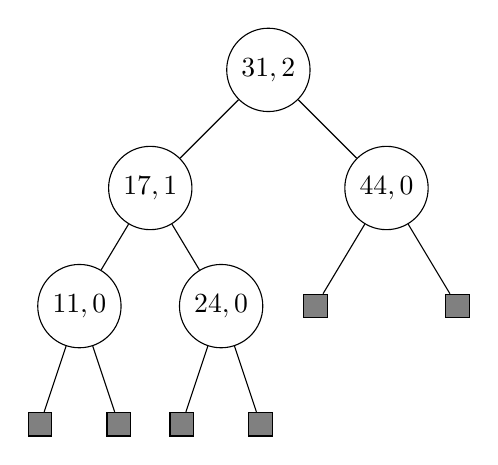
\begin{tikzpicture}[level distance =15mm, baseline=(current bounding box.north)]
\tikzstyle{level 1}=[sibling distance = 30mm]
\tikzstyle{level 2}=[sibling distance = 18mm]
\tikzstyle{level 3}=[sibling distance = 10mm]
\tikzstyle{level 4}=[sibling distance = 10mm]
\tikzstyle{every node}=[circle,draw]
\node {$31,2$}
 child {node{$17,1$}
        child {node{$11,0$} child {node[fl]{}} child {node[fl]{}}}
        child {node{$24,0$} child {node[fl]{}} child {node[fl]{}}}
       }
 child {node{$44,0$} child {node[fl]{}} child {node[fl]{}}
       };
\end{tikzpicture} 
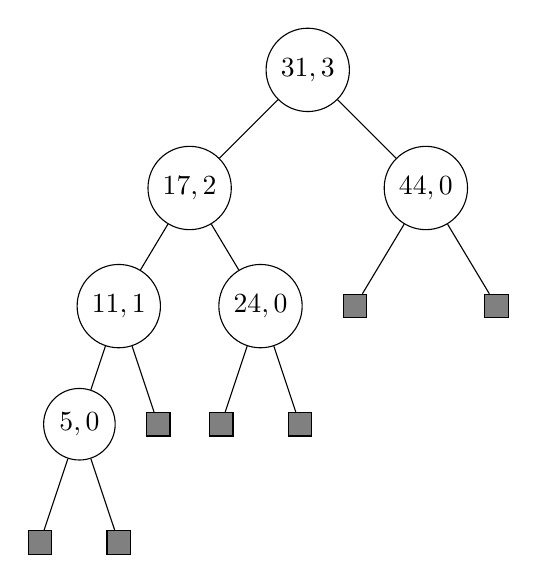
\begin{tikzpicture}[level distance =15mm, baseline=(current bounding box.north)]
\tikzstyle{level 1}=[sibling distance = 30mm]
\tikzstyle{level 2}=[sibling distance = 18mm]
\tikzstyle{level 3}=[sibling distance = 10mm]
\tikzstyle{level 4}=[sibling distance = 10mm]
\tikzstyle{every node}=[circle,draw]
\node {$31,3$}
 child {node{$17,2$}
        child {node{$11,1$}
               child {node{$5,0$} child {node[fl]{}} child {node[fl]{}}}
               child {node[fl]{}}
              }
        child {node{$24,0$} child {node[fl]{}} child {node[fl]{}}}
       }
 child {node{$44,0$} child {node[fl]{}} child {node[fl]{}}};
\end{tikzpicture}
\]
%-------------------------------------------------------------------------------
\medskip

L'arbre n'est alors plus équilibré. Pour en rétablir l'équilibre on va faire tourner la liaison entre la racine et le fils gauche en faisant glisser le fils droit du fils gauche le long de cette liaison pour qu'il devienne le fils gauche de l'ancienne racine devenue fils droit. Cette opération est nommée rotation droite. On définit de même une rotation gauche.
\[
\begin{tikzpicture}[scale=0.9]
\tikzstyle{every node}=[circle,draw,minimum size=8mm]
\tikzstyle{level 1}=[sibling distance =19mm]
\tikzstyle{level 2}=[sibling distance =16mm]
\tikzstyle{level 3}=[sibling distance =13mm]
\tikzstyle{level 4}=[sibling distance =10mm]
  \node {$r$}
   child {node {$n_g$}
          child [child anchor=north]{node[sub]{$gg$}}
          child [child anchor=north]{node[sub]{$gd$}}
         }
   child [child anchor=north]{node[sub]{$d$}};
\end{tikzpicture}
\quad \longrightarrow \quad
\begin{tikzpicture}[scale=0.9]
\tikzstyle{every node}=[circle,draw,minimum size=8mm]
\tikzstyle{level 1}=[sibling distance =19mm]
\tikzstyle{level 2}=[sibling distance =16mm]
\tikzstyle{level 3}=[sibling distance =13mm]
\tikzstyle{level 4}=[sibling distance =10mm]
  \node {$n_g$}
   child [child anchor=north]{node[sub]{$gg$}}
   child {node {$r$}
          child [child anchor=north]{node[sub]{$gd$}}
          child [child anchor=north]{node[sub]{$d$}}
         };
\end{tikzpicture}
\]
On obtient alors un arbre équilibré.

\[
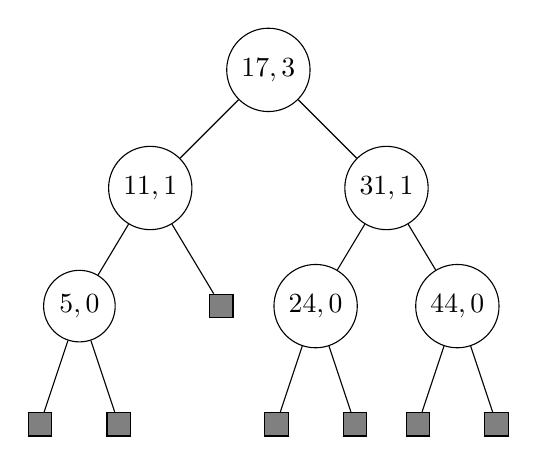
\begin{tikzpicture}[level distance =15mm, baseline=(current bounding box.north)]
\tikzstyle{level 1}=[sibling distance = 30mm]
\tikzstyle{level 2}=[sibling distance = 18mm]
\tikzstyle{level 3}=[sibling distance = 10mm]
\tikzstyle{level 4}=[sibling distance = 10mm]
\tikzstyle{every node}=[circle,draw]
\node {$17,3$}
child {node{$11,1$}
       child {node{$5,0$} child {node[fl]{}} child {node[fl]{}}}
       child {node[fl]{}}
      }
child {node{$31,1$}
       child {node{$24,0$} child {node[fl]{}} child {node[fl]{}}}
       child {node{$44,0$} child {node[fl]{}} child {node[fl]{}}}
      };
\end{tikzpicture} 
\]

\newpage
Par contre si on avait ajouté la valeur 25 à l'arbre initial on aurait obtenu aussi un déséquilibre vers la gauche mais une rotation droite n'aurait fait que le déplacer à droite.
\[
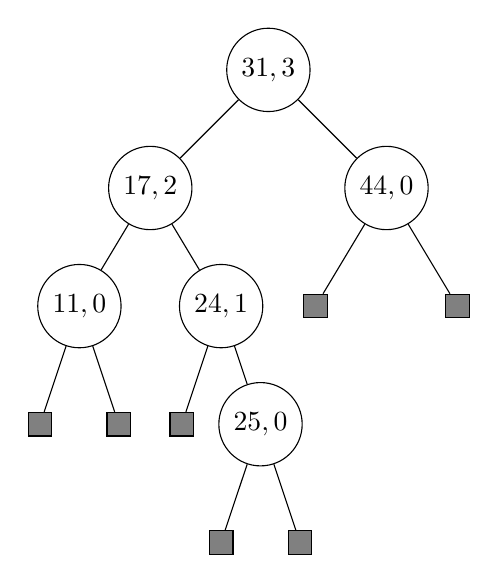
\begin{tikzpicture}[level distance =15mm, baseline=(current bounding box.north)]
\tikzstyle{level 1}=[sibling distance = 30mm]
\tikzstyle{level 2}=[sibling distance = 18mm]
\tikzstyle{level 3}=[sibling distance = 10mm]
\tikzstyle{level 4}=[sibling distance = 10mm]
\tikzstyle{every node}=[circle,draw]
\node {$31,3$}
 child {node{$17,2$}
        child {node{$11,0$} child {node[fl]{}} child {node[fl]{}}}
        child {node{$24,1$} 
               child {node[fl]{}} 
               child {node{$25, 0$} child {node[fl]{}} child {node[fl]{}}}
              }
       }
 child {node{$44,0$} child {node[fl]{}} child {node[fl]{}}
       };
\end{tikzpicture} 
\quad
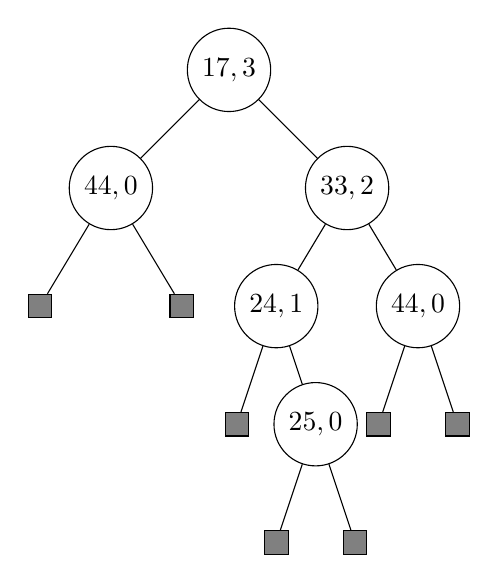
\begin{tikzpicture}[level distance =15mm, baseline=(current bounding box.north)]
\tikzstyle{level 1}=[sibling distance = 30mm]
\tikzstyle{level 2}=[sibling distance = 18mm]
\tikzstyle{level 3}=[sibling distance = 10mm]
\tikzstyle{level 4}=[sibling distance = 10mm]
\tikzstyle{every node}=[circle,draw]
\node {$17,3$}
 child {node{$44,0$} child {node[fl]{}} child {node[fl]{}}}
 child {node{$33,2$}
        child {node{$24,1$}
               child {node[fl]{}}
               child {node{$25,0$} child {node[fl]{}} child {node[fl]{}}}
              }
        child {node{$44,0$} child {node[fl]{}} child {node[fl]{}}}
       };
\end{tikzpicture}
\]
La solution est d'effectuer une rotation gauche sur le fils gauche avant de réaliser la rotation droite.
\[
\begin{tikzpicture}[scale=0.9]
\tikzstyle{every node}=[circle,draw,minimum size=8mm]
\tikzstyle{level 1}=[sibling distance =19mm]
\tikzstyle{level 2}=[sibling distance =16mm]
\tikzstyle{level 3}=[sibling distance =13mm]
\tikzstyle{level 4}=[sibling distance =10mm]
  \node {$r$}
   child {node {$n_g$}
          child [child anchor=north]{node[sub]{$gg$}}
          child {node {$n_{gd}$}
                 child [child anchor=north]{node[sub]{$gdg$}}
                 child [child anchor=north]{node[sub]{$gdg$}}
                }
         }
   child [child anchor=north]{node[sub]{$d$}};
\end{tikzpicture}
\quad \longrightarrow \quad
\begin{tikzpicture}[scale=0.9]
\tikzstyle{every node}=[circle,draw,minimum size=8mm]
\tikzstyle{level 1}=[sibling distance =19mm]
\tikzstyle{level 2}=[sibling distance =16mm]
\tikzstyle{level 3}=[sibling distance =13mm]
\tikzstyle{level 4}=[sibling distance =10mm]
  \node {$r$}
   child {node {$n_{gd}$}
          child {node {$n_{g}$}
                 child [child anchor=north]{node[sub]{$gg$}}
                 child [child anchor=north]{node[sub]{$gdg$}}
                }
          child [child anchor=north]{node[sub]{$gdd$}}
         }
   child [child anchor=north]{node[sub]{$d$}};
\end{tikzpicture}
\quad \longrightarrow \quad
\begin{tikzpicture}[scale=0.9]
\tikzstyle{every node}=[circle,draw,minimum size=8mm]
\tikzstyle{level 1}=[sibling distance =32mm]
\tikzstyle{level 2}=[sibling distance =16mm]
\tikzstyle{level 3}=[sibling distance =13mm]
\tikzstyle{level 4}=[sibling distance =10mm]
  \node {$n_{gd}$}
  child {node {$n_{g}$}
         child [child anchor=north]{node[sub]{$gg$}}
         child [child anchor=north]{node[sub]{$gdg$}}
        }
   child {node {$r$}
          child [child anchor=north]{node[sub]{$gdd$}}
          child [child anchor=north]{node[sub]{$d$}}
         }
;
\end{tikzpicture}
\]

On parvient ainsi à un arbre équilibré
\[
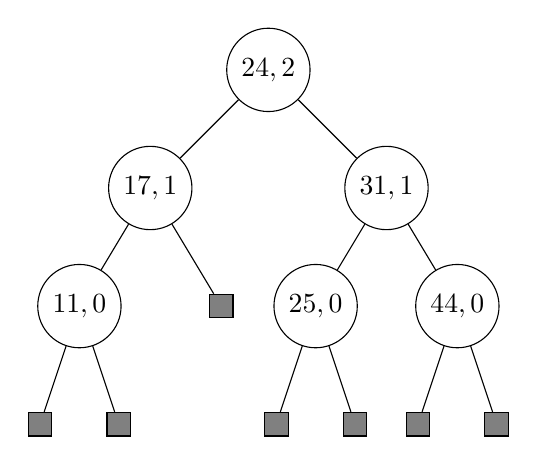
\begin{tikzpicture}[level distance =15mm, baseline=(current bounding box.north)]
\tikzstyle{level 1}=[sibling distance = 30mm]
\tikzstyle{level 2}=[sibling distance = 18mm]
\tikzstyle{level 3}=[sibling distance = 10mm]
\tikzstyle{level 4}=[sibling distance = 10mm]
\tikzstyle{every node}=[circle,draw]
\node {$24,2$}
 child {node{$17,1$}
        child {node{$11,0$} child {node[fl]{}} child {node[fl]{}}}
        child {node[fl]{}} 
       }
 child {node{$31,1$} 
        child {node{$25,0$} child {node[fl]{}} child {node[fl]{}}}
        child {node{$44,0$} child {node[fl]{}} child {node[fl]{}}}
       };
\end{tikzpicture} 
\]
%--------------------------------------------------------------------------

Dans la pratique on n'équilibre pas l'arbre après l'avoir construit : on le construit équilibré.
%--------------------------------------------------------------------------
%--------------------------------------------------------------------------
\begin{Exercise}\it 
Écrire une fonction \type{noeud g n0 d} avec $n_0$ valeur et $g$ et $d$ deux arbres AVL dont les hauteurs diffèrent de 2 au plus en valeur absolue, renvoie un arbre AVL  contenant les valeurs des deux arbres ainsi que $n_0$.
\end{Exercise}
%--------------------------------------------------------------------------
\begin{Answer} 
\begin{lstlisting}
let noeud g n0 d =
  let hg = ht g in
  let hd = ht d in
  match (hg - hd) with
  |2 -> begin match g with
    |Noeud(gg, rg, gd, _) when ht gg >= ht gd 
      -> cons gg rg (cons gd n0 d)
    |Noeud(gg, rg, Noeud(gdg, rgd, gdd, _), _)
      -> cons (cons gg rg gdg) rgd (cons gdd n0 d)
    | _ -> failwith "Ceci ne devrait pas arriver" end
  |(-2) -> begin match d with
    |Noeud(dg, rd, dd, _) when ht dd > ht dg
      -> cons (cons g n0 dg) rd dd
    |Noeud(Noeud(dgg, rdg, dgd, _), rd, dd, _) 
      -> cons (cons g n0 dgg) rdg (cons dgd rd dd)
    | _ -> failwith "Ceci ne devrait pas arriver" end
  | _ -> cons g n0 d;;
\end{lstlisting}
\newpage
\end{Answer}
%--------------------------------------------------------------------------
%-------------------------------------------------------------------------------
\subsection{Arbres binaires de recherche}
%--------------------------------------------------------------------------
%--------------------------------------------------------------------------
On remarque qu'une rotation d'un arbre binaire de recherche donne un arbre binaire de recherche ; une démonstration possible consiste à prouver que le parcours infixe est inchangé.

La construction ci-dessus permet donc de maintenir un arbre binaire de recherche.

Dans la suite on désignera un arbre binaire de recherche AVL équilibré simplement sous le nom {\bf arbre AVL}.
%--------------------------------------------------------------------------
%--------------------------------------------------------------------------
\begin{Exercise}\it 
Écrire une fonction \type{insertion n arbre} qui reçoit une valeur et un arbre AVL et qui renvoie un arbre AVL contenant les valeurs de l'arbre ainsi que $n_0$. On insérera la valeur dans une feuille. Si la valeur existait déjà dans l'arbre on renvoie le même arbre.
\end{Exercise}
%--------------------------------------------------------------------------
\begin{Answer} 
\begin{lstlisting}
let rec insertion n arbre = 
  match arbre with
  |Vide -> feuille n
  |Noeud(g, r, d, h) when n = r -> arbre
  |Noeud(g, r, d, h) when n < r
                  -> noeud (insertion n g) r  d
  |Noeud(g, r, d, h) -> noeud g r (insertion n d);;
\end{lstlisting}
\end{Answer}
%--------------------------------------------------------------------------
%--------------------------------------------------------------------------
\begin{Exercise}\it 
Écrire une fonction qui reçoit une liste de valeurs et qui affiche les arbres AVL construits en ajoutant successivement les valeurs de la liste à partir de l'arbre vide.
\end{Exercise}
%--------------------------------------------------------------------------
\begin{Answer} 
\begin{lstlisting}
let evolution liste =
  let rec aux liste arbre =
    match liste with
    |[] -> ()
    |n::reste -> let a1 = insertion n arbre in
                 let _ = dessin a1 x0 y0 in
                 clear_graph();
                 aux reste a1 in
  aux liste Vide;
  close_graph();;
\end{lstlisting}
\end{Answer}
%--------------------------------------------------------------------------
%--------------------------------------------------------------------------
\begin{Exercise}\it 
Écrire une fonction \type{suppression n arbre} qui reçoit une valeur et un arbre AVL et qui renvoie un arbre AVL contenant les valeurs de l'arbre à l'exception de $n_0$ s'il était présent.
\end{Exercise}
%--------------------------------------------------------------------------
\begin{Answer} 
\begin{lstlisting}
let rec maxArbre arbre = 
  match arbre with
  |Vide -> raise(Failure "Arbre vide")
  |Noeud(_, r, Vide, _) -> r
  |Noeud(_, _, d, _) -> maxArbre d;;

let rec suppressionMax arbre = 
  match arbre with
  |Vide -> failwith "Arbre vide"
  |Noeud(g, r, Vide, h) -> g
  |Noeud(g, r, d, h) -> noeud g r (suppressionMax d);;

let suppressionRacine arbre = 
  match arbre with
  |Vide -> Vide
  |Noeud(Vide, r, d, h) -> d
  |Noeud(g, r, d, h) ->  let p = maxArbre g in
                      noeud (suppressionMax g) p d;;

let rec suppression n arbre = 
  match arbre with
  |Vide -> Vide
  |Noeud(g, r, d, h) when n = r 
                     -> suppressionRacine arbre
  |Noeud(g, r, d, h) when n < r 
                     -> noeud (suppression n g) r d
  |Noeud(g, r, d, h) -> noeud g r (suppression n d);;
\end{lstlisting}

\newpage
\end{Answer}
%--------------------------------------------------------------------------
%--------------------------------------------------------------------------
\begin{Exercise}\it 
Qu'est-ce qui rend difficile l'insertion à la racine ?

Proposer une fonction.
\end{Exercise}
%--------------------------------------------------------------------------
\begin{Answer} 
Lors du découpage d'un arbre on peut obtenir deux arbres dont la différence de hauteur est supérieure à 2. Pour pouvoir équilibrer on peut remplacer la fonction \type{noeud} en rendant récursive et en traitant les cas de différences supérieures ou égales à 2 en valeur absolue.

\begin{lstlisting}
let rec noeud g n0 d =
  let hg = ht g in
  let hd = ht d in
  if (hg - hd) > 1
  then begin match g with
    |Noeud(gg, rg, gd, _) when ht gg >= ht gd 
      -> noeud gg rg (noeud gd n0 d)
    |Noeud(gg, rg, Noeud(gdg, rgd, gdd, _), _)
      -> noeud (noeud gg rg gdg) rgd (noeud gdd n0 d)
    | _ -> failwith "Ceci ne devrait pas arriver" end
  else if (hg - hd) < -1 
  then begin match d with
    |Noeud(dg, rd, dd, _) when ht dd > ht dg
      -> cons (cons g n0 dg) rd dd
    |Noeud(Noeud(dgg, rdg, dgd, _), rd, dd, _) 
      -> cons (cons g n0 dgg) rdg (cons dgd rd dd)
    | _ -> failwith "Ceci ne devrait pas arriver" end
  else cons g n0 d;;
\end{lstlisting}

\begin{lstlisting}
let rec decoupage n arbre = 
  match arbre with
  |Vide -> (Vide,Vide)
  |Noeud(g, r, d, h) when n = r -> (g, d)
  |Noeud(g, r, d, h) when n < r
                     -> let (gg, gd) = decoupage n g 
                         in (gg, noeud gd r d)
  |Noeud(g, r, d, h) -> let (dg, dd) = decoupage n d 
                        in (noeud g r dg, dd);;

let insertionRacine n arbre =
  let (g, d)= decoupage n arbre
  in noeud g n d;;
\end{lstlisting}
\end{Answer}
%--------------------------------------------------------------------------
%-------------------------------------------------------------------------------


%-------------------------------------------------------------------------------
%-------------------------------------------------------------------------------
%-------------------------------------------------------------------------------
